\documentclass[
fontsize=12pt,					% Schriftgröße
paper=a4,						% Papierformat
twoside=false, 					% einseitiges (false) oder zweiseitiges (true) Dokument
listof=totoc, 					% Tabellen- und Abbildungsverzeichnis ins Inhaltsverzeichnis
bibliography=totoc,				% Literaturverzeichnis ins Inhaltsverzeichnis aufnehmen
titlepage, 						% Titlepage-Umgebung statt \maketitle
headsepline, 					% horizontale Linie unter Kolumnentitel
%abstracton,					% Überschrift beim Abstract einschalten, Abstract muss dazu in {abstract}-Umgebung stehen
DIV=12,							% Satzspiegeleinstellung, 12 ist Standar bei KOMA
BCOR=6mm,						% Bindekorrektur, die den Seitenspiegel um 3mm nach rechts verschiebt,
cleardoublepage=empty,			% Stil einer leeren eingefügten Seite bei Kapitelwechsel
parskip,							% Absatzabstand bei Absatzwechsel einfügen
ngerman
]{scrartcl}

\usepackage[setspace=false]{scrhack}
\usepackage[utf8]{inputenc} 	% ermöglicht die direkte Eingabe von Umlauten
\usepackage[T1]{fontenc} 		% Ausgabe aller zeichen in einer T1-Codierung (wichtig für die Ausgabe von Umlauten!)
\usepackage{babel} 	% deutsche Trennungsregeln und Übersetzung der festcodierten Überschriften
\renewcaptionname{ngerman}{\contentsname}{Inhaltsverzeichnis}
\renewcaptionname{ngerman}{\bibname}{Literaturverzeichnis}
\setlength{\parindent}{0ex} 	% bei neuem Abschnitt nicht einrücken

\newcommand{\lowrule}{%
	\leavevmode \kern.06em\vbox{\hrule width.5em}}

\usepackage{siunitx}			% Vereinfachte Eingabe von Einheiten in Formeln
\sisetup{
	number-unit-product = \;,
	inter-unit-product = \:,
	exponent-product = \cdot,
	output-decimal-marker = {,}
}

\usepackage{graphicx}  			% Einbinden von Grafiken erlauben
\usepackage[format=hang,		% Formatierungen von Unter- / Überschriften
font=normal,
labelfont=bf,
justification=RaggedRight,
singlelinecheck=true,
aboveskip=1mm
]{caption}

\usepackage[backend=biber, %% Hilfsprogramm "biber" beim Compilieren nutzen (statt "biblatex" oder "bibtex")
style=numeric, %% Zitierstil (siehe Dokumentation)
natbib=true, %% Bereitstellen von natbib-kompatiblen Zitierkommandos
hyperref=true, %% hyperref-Paket verwenden, um Links zu erstellen
]{biblatex}
\addbibresource{literature/lit.bib}

\usepackage{pdfpages}

\usepackage{enumitem}			% Erlaubt Änderung der Nummerierung in der Umgebung enumerate

\usepackage{amsmath}			% Ergänzungen für Formeln
\usepackage{textcomp} 			% zum Einsatz von Eurozeichen u. a. Symbolen
\usepackage{eurosym}			% bessere Darstellung Euro-Symbol mit \euro

\usepackage[					% Einstellunge Paket hyperref
hyperfootnotes=false,			% im pfd-Output Fußnoten nicht verlinken
hidelinks						% Entfernen von farbigen Umrandungen der Links
]{hyperref}

\usepackage[					% Einstellungen für Fußnoten
bottom,							% Ausrichtung unten
multiple,						% Trennung durch Seperator bei mehreren Fußnoten
hang,
marginal
]{footmisc}

\usepackage{calc}				% Paket zum Berechnen von Längen z.B. 0.8\linewidth

\usepackage{xcolor} 			% einfache Verwendung von Farben in nahezu allen Farbmodellen

\usepackage{listings}			% Darstellung von Quellcode mit den Umgebungen {lstlisting}, \lstinline und \lstinputlisting
\lstset{literate=				% Damit können Umlaute innerhalb Listings geschrieben werden
	{Ö}{{\"O}}1
	{Ä}{{\"A}}1
	{Ü}{{\"U}}1
	{ß}{{\ss}}1
	{ü}{{\"u}}1
	{ä}{{\"a}}1
	{ö}{{\"o}}1
}
\definecolor{mygreen}{rgb}{0,0.6,0}
\definecolor{mygray}{rgb}{0.5,0.5,0.5}
\definecolor{mymauve}{rgb}{0.58,0,0.82}
\lstset{ %
	backgroundcolor=\color{white},   % choose the background color; you must add \usepackage{color} or \usepackage{xcolor}; should come as last argument
	basicstyle=\footnotesize,        % the size of the fonts that are used for the code
	breakatwhitespace=false,         % sets if automatic breaks should only happen at whitespace
	breaklines=true,                 % sets automatic line breaking
	captionpos=t,                    % sets the caption-position to (b) bottom or (t) top
	commentstyle=\color{mygreen},    % comment style
	deletekeywords={...},            % if you want to delete keywords from the given language
	escapeinside={\%*}{*)},          % if you want to add LaTeX within your code
	escapeinside={(*@}{@*)},
	extendedchars=true,              % lets you use non-ASCII characters; for 8-bits encodings only, does not work with UTF-8
	frame=none,	                   	% "single" adds a frame around the code; "none"
	keepspaces=true,                 % keeps spaces in text, useful for keeping indentation of code (possibly needs columns=flexible)
	keywordstyle=\color{blue},       % keyword style
	language=[LaTeX]TeX,             % the language of the code
	morekeywords={*,nomenclature},   % if you want to add more keywords to the set
	numbers=left,                    % where to put the line-numbers; possible values are (none, left, right)
	numbersep=5pt,                   % how far the line-numbers are from the code
	numberstyle=\tiny\color{mygray}, % the style that is used for the line-numbers
	rulecolor=\color{black},         % if not set, the frame-color may be changed on line-breaks within not-black text (e.g. comments (green here))
	showspaces=false,                % show spaces everywhere adding particular underscores; it overrides 'showstringspaces'
	showstringspaces=false,          % underline spaces within strings only
	showtabs=false,                  % show tabs within strings adding particular underscores
	stepnumber=1,                    % the step between two line-numbers. If it's 1, each line will be numbered
	stringstyle=\color{mymauve},     % string literal style
	tabsize=2,	                   % sets default tabsize to 2 spaces
	title=\lstname                   % show the filename of files included with \lstinputlisting; also try caption instead of title
}

% Folgende Zeilen definieren Abkürzungen, um Befehle schneller eingeben zu können
\newcommand{\ua}{\mbox{u.\,a.\ }}
\newcommand{\zB}{\mbox{z.\,B.\ }}
\newcommand{\bs}{$\backslash$}
\newcommand*\diff{\mathop{}\!\mathrm{d}}	% Differentialzeichen
\newcommand*\Diff[1]{\mathop{}\!\mathrm{d^#1}} % Differentialzeichen höherer Ableitung
\newcommand*\jj{\mathop{}\!\mathrm{j}}	% Komplexe Zahl j

% Folgende Zeilen weden benötigt, um Tikz und PGF-Plot-Grafiken einzubinden
\usepackage{pgfplots}
\usepackage{pgfplotstable}
\pgfplotsset{compat=newest,width=0.6\linewidth}
\usepgfplotslibrary{smithchart}
\usepackage{tikz}						% Tikz sollte nach Listings Pakete geladen werden.
\usetikzlibrary{arrows}

\hyphenation{Schrift-ar-ten}

\BeforeClosingMainAux{% siehe KOMA-Script-Anleitung
	\addcontentsline{toc}{chapter}{\indexname}\stepcounter{page}
}

%opening
\title{Prüfungsleistung in \glqq Digitale Bildverarbeitung und Mustererkennung\grqq}
\subtitle{Dokumentation}
\author{Tim Lucas Halt (MatrNr. 6682645)}

\begin{document}

\maketitle

\section{Methodik}

Die Arbeit gliedert sich in zwei Teile. Der Erste enthält Versuche mit dem MNIST-Datensatz. Der Zweite einige Experimente mit dem TinySchiller-Datensatz\\
Bei MNIST wird primär eine hohe maximale Genauigkeit durch automatisierte Untersuchungen angestrebt. Als Tool wird dafür Weigts\&Biases \autocite{wandb.sweep} verwendet. Es ermöglicht automatische Sweeps, sowie Werkzeuge zur Analyse und Dokumentation. Alle Untersuchungen gehen von dem Netz in \autoref{basis} aus, mit dem der erste Accuracy-Benchmark gesetzt wurde. Im ersten Schritt werden die Hyperparameter optimiert. Um möglichst viele automatisiert Kombinationen zu testen, wird GPU-Rechenleistung von Kaggle und Colab verwendet. Als Zweites werden die Callback in das Training integriert, gefolgt von einer Data-Augmentation. Die endgültige Qualität wird anhand einer Versuchsreihe mit \textcolor{red}{XY} Trainings ermittelt.\\
Abschließend werden Versuche gezeigt, zur Reduktion der Label- und Parameter-Anzahl und Ergebnisse mit dem TinySchiller-Datensatz.

\section{MNIST}

\subsection{Grundlage}
\label{sec:basis}

Das Ausgangsnetz, von dem die Betrachtungen ausgehen ist in \autoref{basis} dargestellt. Es hat etwa 62-tausend Parameter. Kompiliert mit dem Adam Optimizer, einer Learning-Rate von 0.003 und einem Training mit dem vollständigen Trainingsdatensatz (60000 Label) bei einer Batch-Size von 512 über 100 Epochen erreichte es 99,47\% Genauigkeit.

\begin{lstlisting}[language=Python, caption=Grundlagen-Netz, label=basis]
	InputLayer(input_shape=(28,28,1)),
	Conv2D(filter=28, kernel_size=5, padding='same', activation='relu'),
	MaxPooling2D(2,2),
	Dropout(0.2),
	Conv2D(filter=16, kernel_size=5, padding='same', activation='relu'),
	MaxPooling2D(2,2),
	Dropout(0.2),
	Flatten(),
	Dense(64, kernel_regularizer = tf.keras.regularizers.l2(0.07), activation = 'relu'),
	Dropout(0.2),
	GaussianNoise(0.1),
	Dense(10, activation='softmax')
\end{lstlisting}

\subsection{Dimensionierung der Filter- und Neuronen-Anzahl}

\begin{figure}
	\centering
	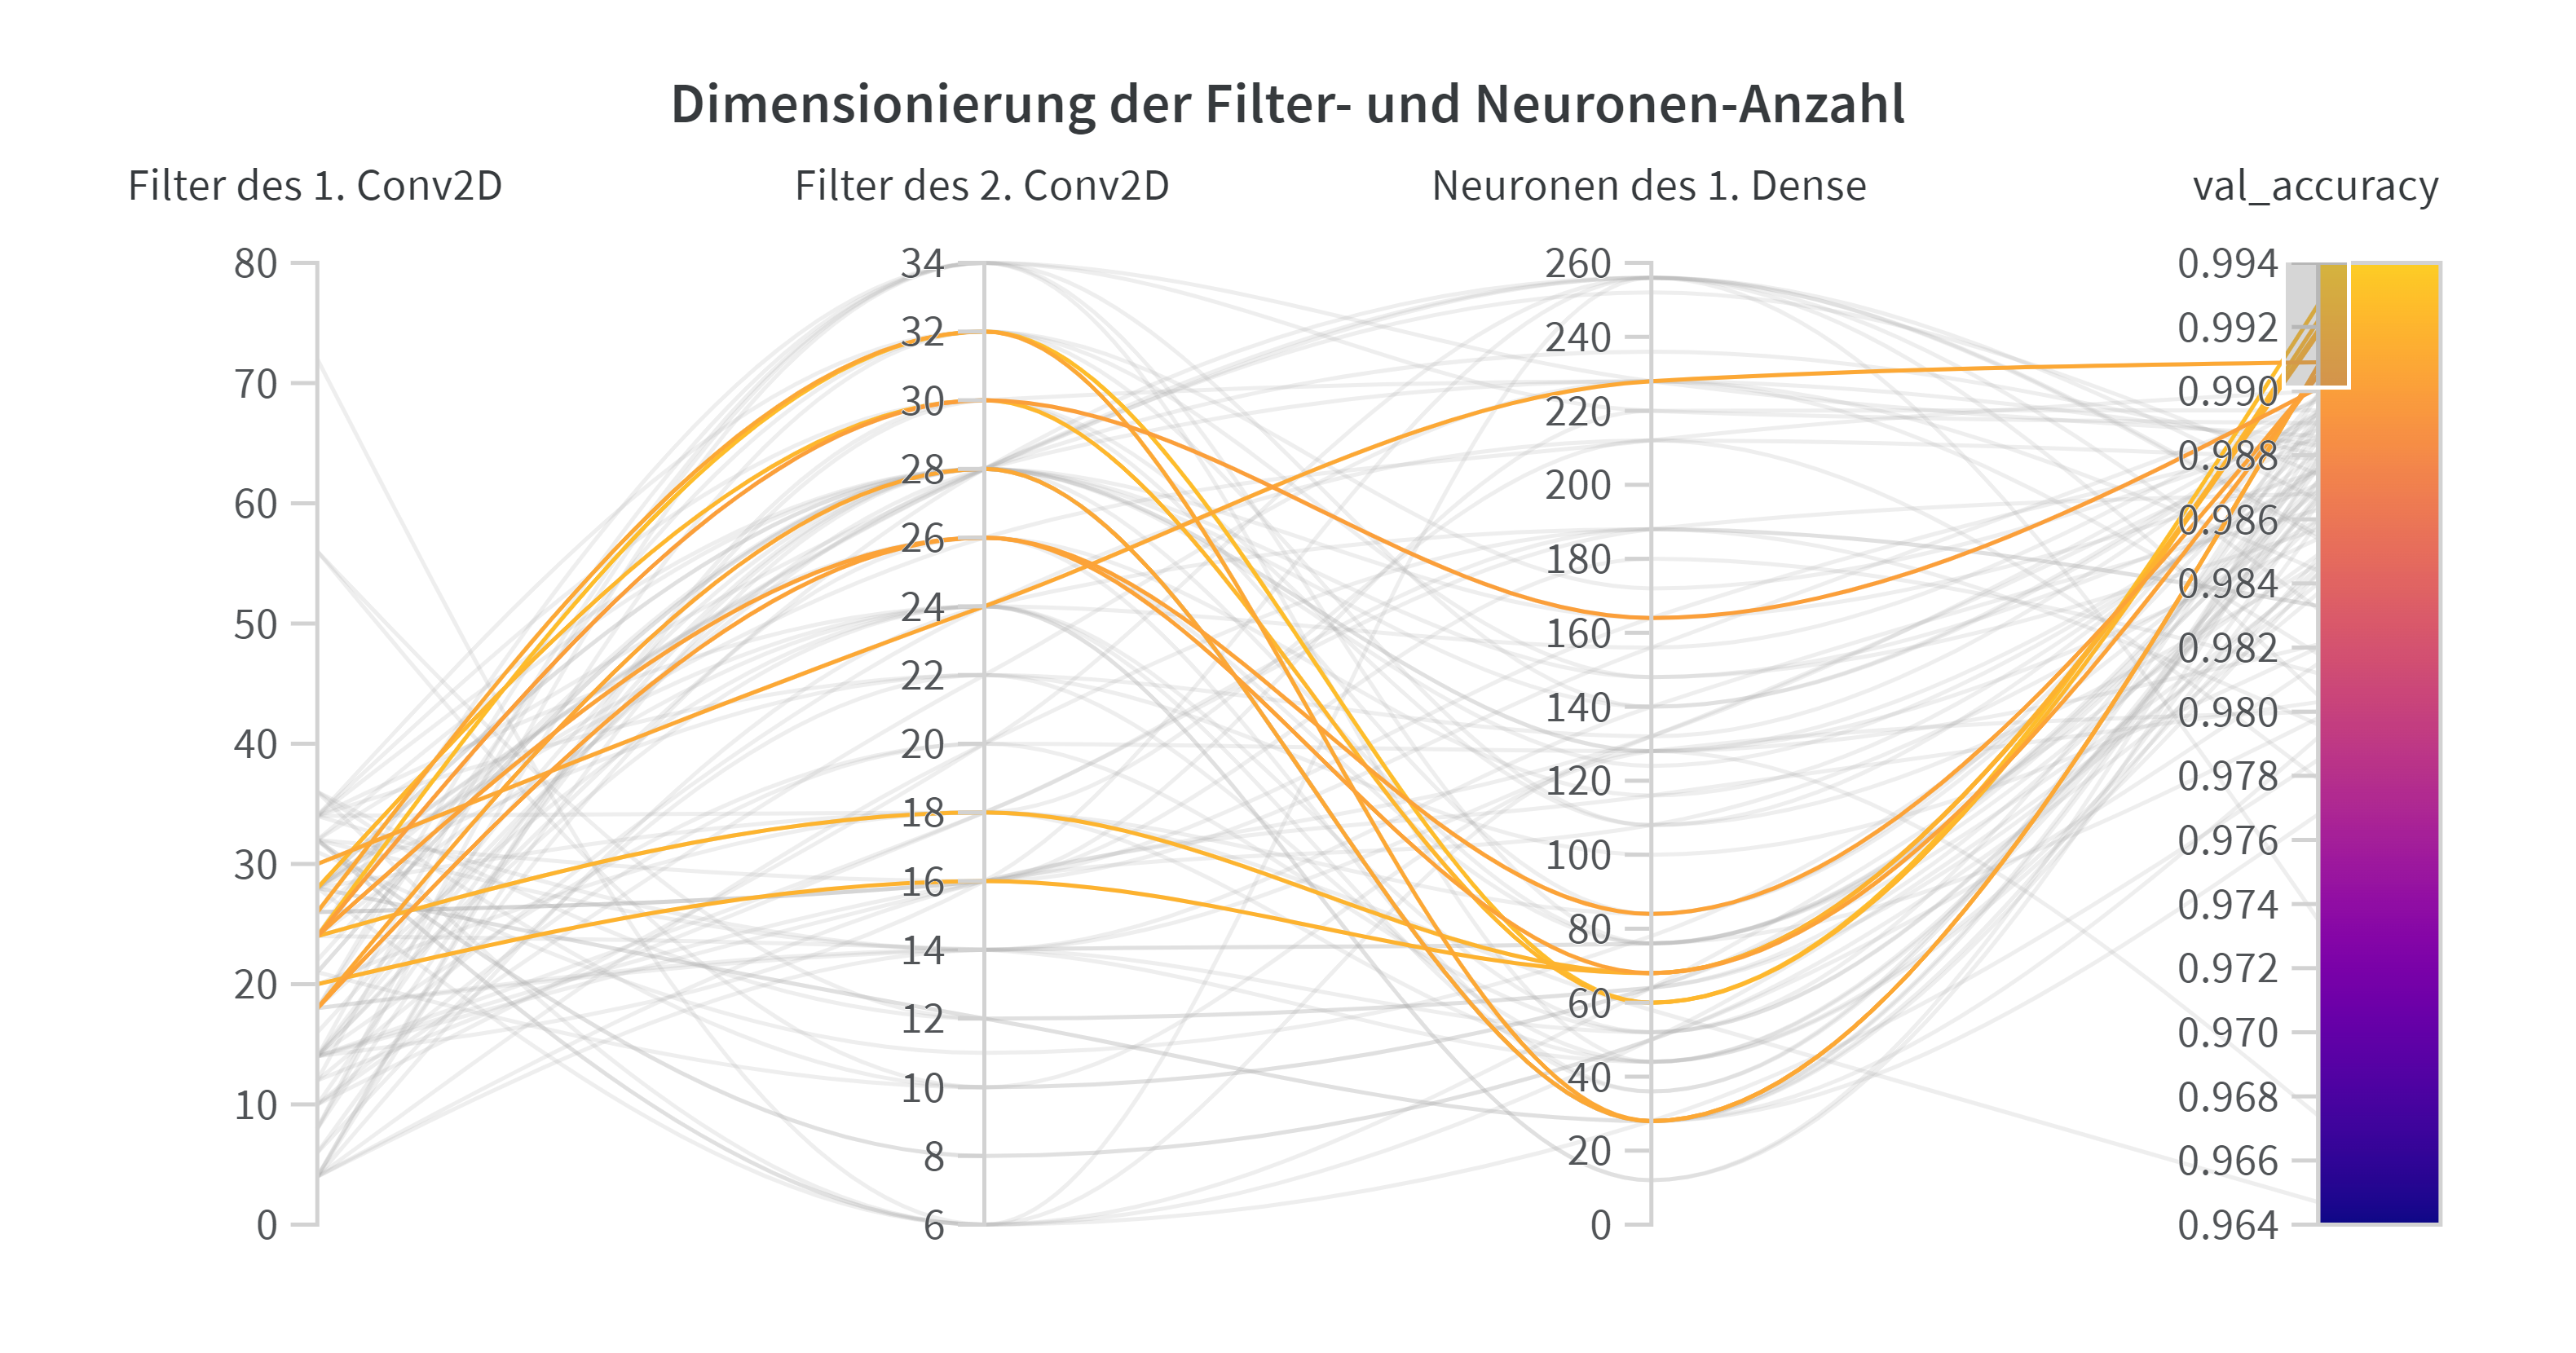
\includegraphics[width=0.7\linewidth]{images/Filter}
	\caption{Etwa 100 Kombinationen aus Filter- und Neuronen-Anzahlen bewertet nach der val\_accuracy. Dokumentiert mit Weight \& Biases}
	\label{fig:filter}
\end{figure}

Zunächst erfolgt die Untersuchung der Filter-Anzahlen in den Convolution-Layern und der Neuronen-Anzahl des ersten Dense-Layer. Das Output-Dense-Layer wird bei 10 Neuronen und der \emph{softmax}-Aktivierungsfunktion belassen, damit jeder Klasse eine Wahrscheinlichkeit zugeordnet wird.\\
Als Methode ist in Weights\&Biases \emph{bayes}, die Bayes'sche Optimierung, zur Maximierung der val\_accuracy gewählt. Dabei werden die Hyperparameter aus einem vorgegebenen Raster gewählt, ein Training durchgeführt und die Ergebnisse dokumentiert. Das Raster für die Filter und Neuronen wurde so gewählt, dass (1) eine Abstufung im Convolution-Teil erfolgt, (2) auch Zahlen nicht zur Basis zwei getestet werden und (3) die Parameteranzahl nicht exorbitant groß wird. Das erste Kriterium erwies sich als kontraproduktiv und wird später verworfen.\\
Die Ergebnisse von circa 100 Kombinationen sind in \autoref{fig:filter} dargestellt. Hervorgehoben sind die besten Zehn. Nach weiter eingegrenztem Sweeps sind in beiden Convolution-Layern 28 Filter gewählt und 54 Neuronen für das Dense-Layer. Den Quellcode des Testes enthält die Datei \emph{pepsi.wandb}.\\

\subsection{Wahl der Aktivierungsfunktionen}

Für die Wahl der Aktivierungsfunktionen wurden ebenfalls Sweeps durchgeführt. Die Ergebnisse sind in \autoref{fig:activ} abgebildet und die besten fünf hervorgehoben. Sie haben die Sigmoid-Funktion im Dense-Layer gemeinsam. Bei den Convolution-Layern zeigte über alle Kombinationen hinweg die Relu-Funktion die stärkste Tendenz zu hoher Genauigkeit. Entsprechend wurde gewählt: Relu, Relu, Sigmoid.

\begin{figure}[h]
	\centering
	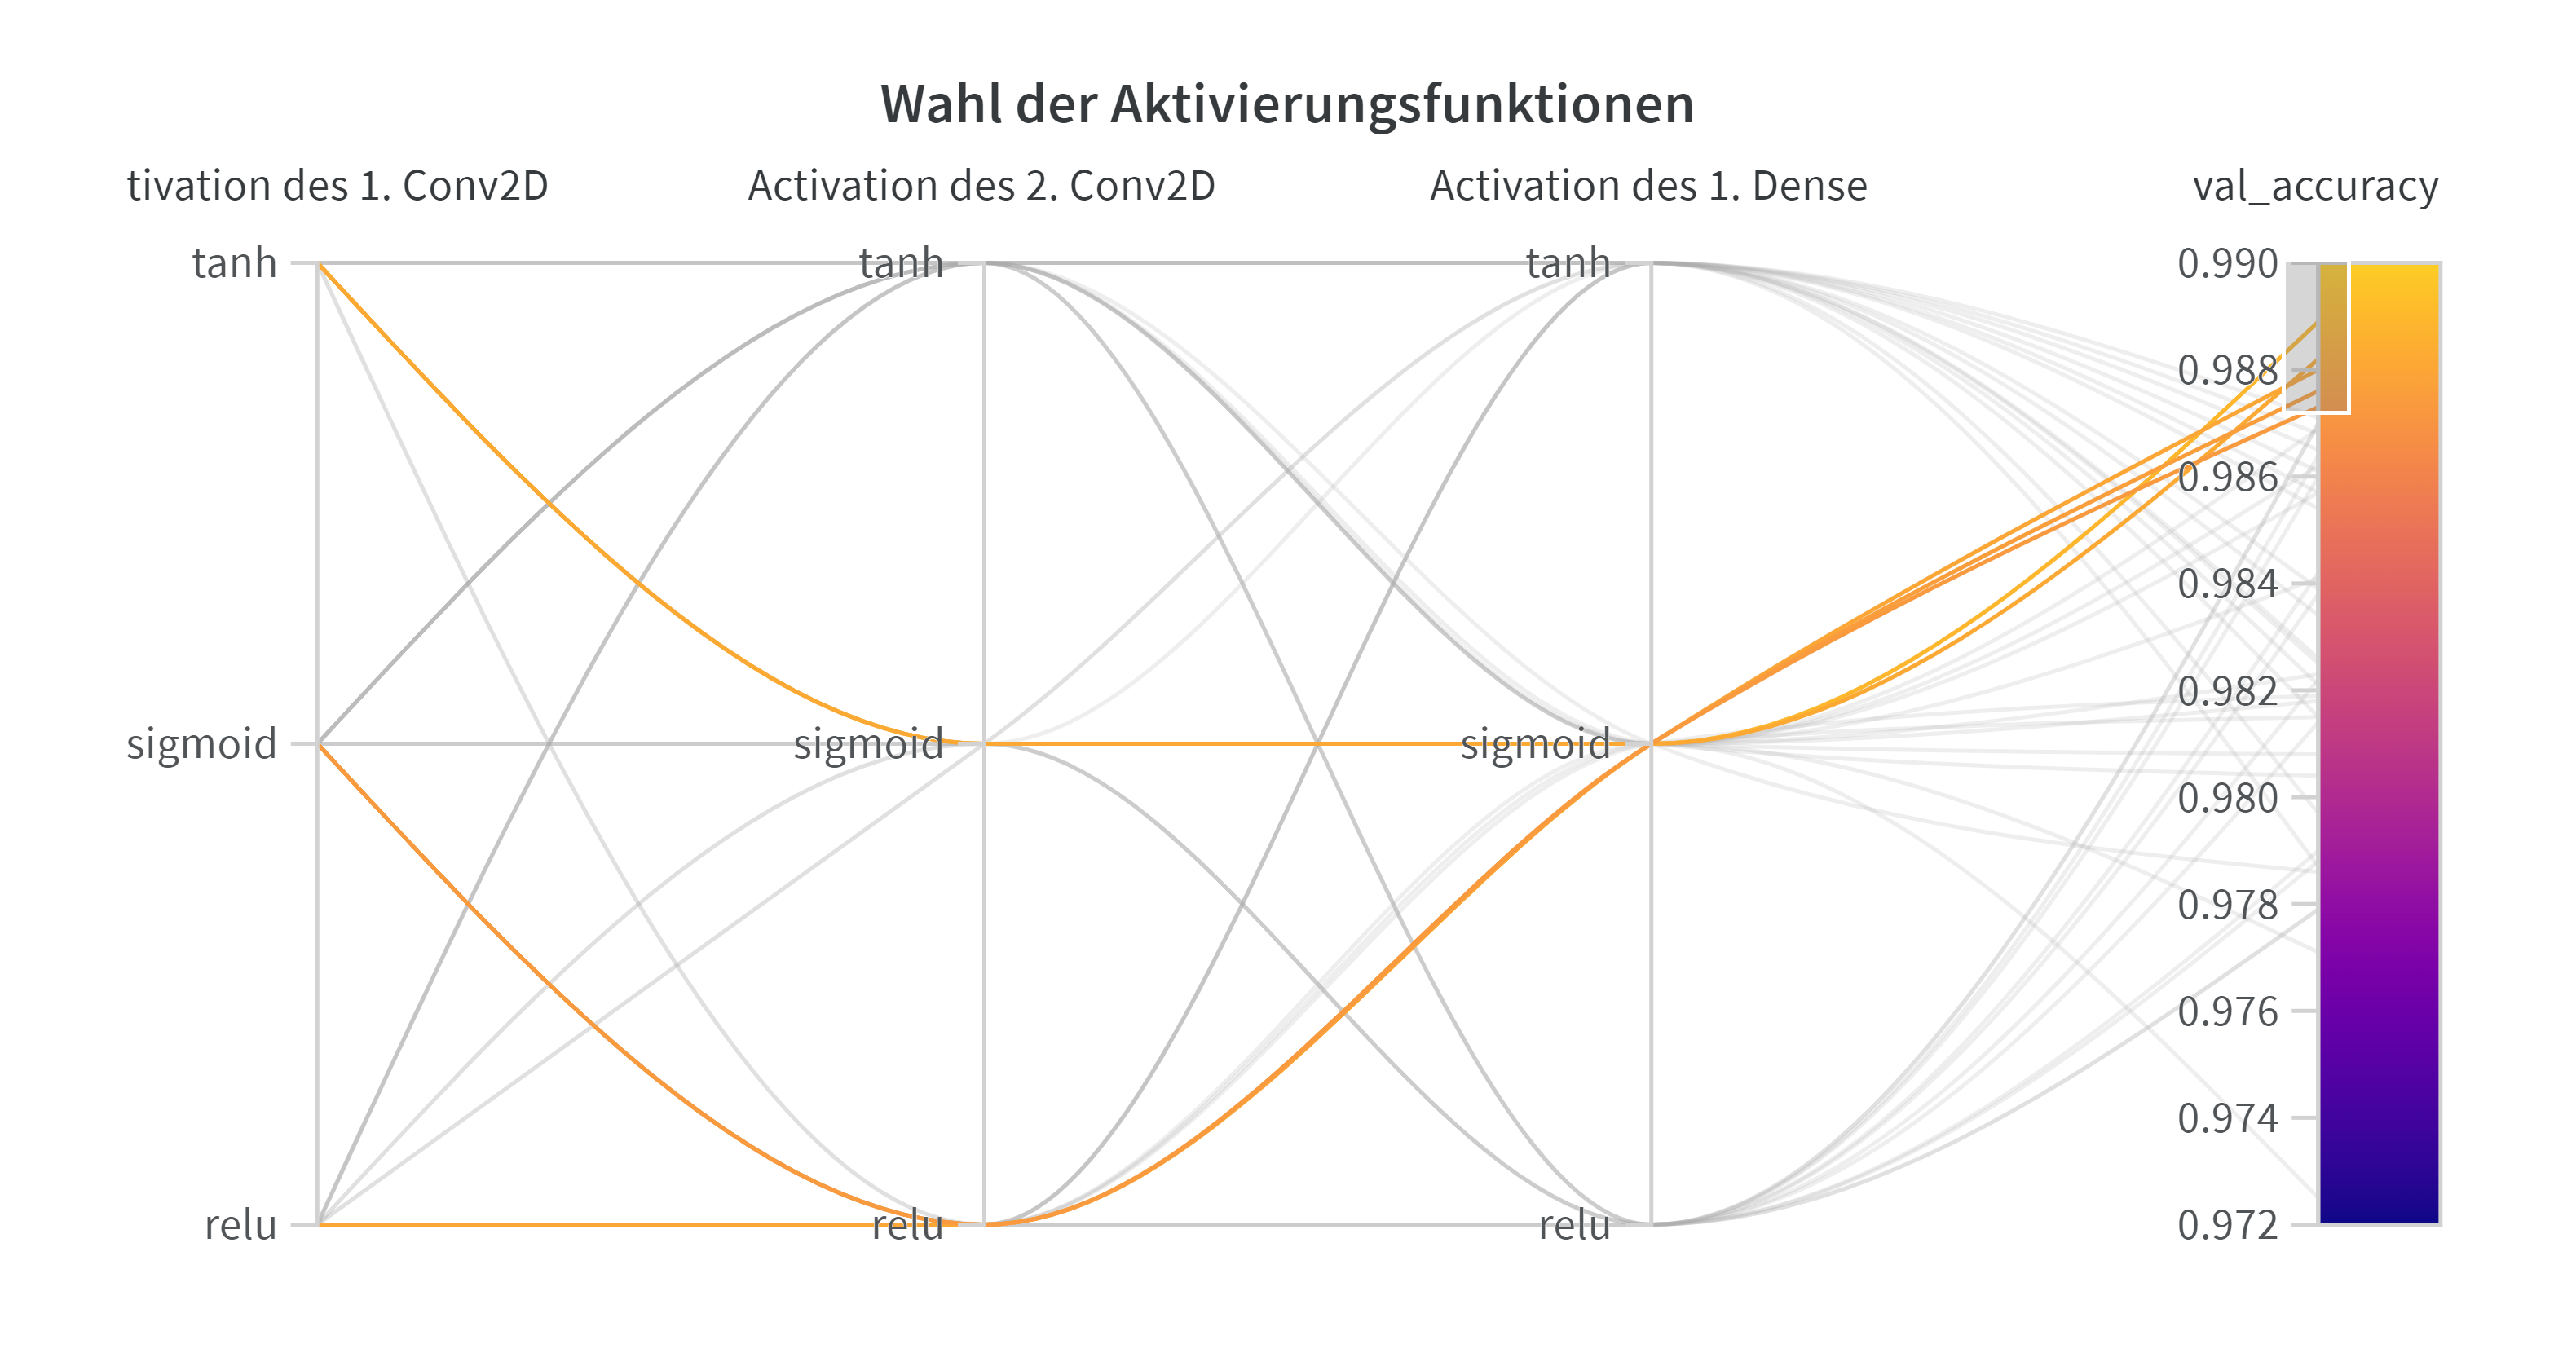
\includegraphics[width=0.7\linewidth]{images/Activ}
	\caption{Kombinationen der Aktivierungsfunktionen bewertet nach der val\_accuracy. Dokumentiert mit Weight \& Biases}
	\label{fig:activ}
\end{figure}

\subsection{BatchNormalization, Dropout und GaussianNoise}

Als drittes wird das Netz um BatchNormalization vor den MaxPool und Dropout erweitert, um das Model zu stabilisieren. Bei anderen Reihenfolgen kommt es zu Widersprüchen \autocite{Li.2018} Anschließend wurden die Dropout- und GaussianNoise-Werte getestet, ebenfalls mit Weigts \& Biasses. Als erfolgreich erwiesen sich Dropouts von 0,4 und GaussianNoise von 0,75. \autocite{Cai.2020}.

\subsection{Callbacks - Early Stopping und Variable Learning Rate}

Nach der Optimierung der Hyperparameter des Netzes, wird der Trainingsprozess verbessert, indem er mit Callbacks angereichert wird. Zum einen wird EarlyStopping eingesetzt, um wenig erfolgreiche Trainings abzubrechen. Um darüber hinaus schneller den Grenzwert zu erreichen wird eine Variable Learning Rate verwendet. In Kombination mit dem EarlyStopping zeigte eine gleichmäßige Reduktion mit jeder Epoche bessere Ergebnisse, als die Methode ReduceLROnPlateau. In Kombination mit einer Batch Size von 32 ergaben sich die besten Ergebnisse

\begin{lstlisting}[language=Python, caption=Callbacks, label=callback]
	er = EarlyStopping(
		monitor="val_accuracy",
		patience=10,
	    restore_best_weights=True
	)
	vlr = LearningRateScheduler(lambda x: 1e-3 * 0.995 ** x)
\end{lstlisting}

\subsection{Data Augmentation}

Die Anzahl an Trainingsdaten wird mit einer Augmentation erweitert. Dazu kommt der ImageDataGenerator von Keras zum Einsatz. Wie er \autoref{da} zu entnehmen ist. Die Bilder werden nicht gespiegelt, weil die Zahlen nicht entsprechend symmetrisch sind. Die gewählten Werte wurden ebenfalls mit Weight\&Biases Sweeps getestet.

\begin{lstlisting}[language=Python, caption=Data Augmentation, label=da]
	
	datagen = tf.keras.preprocessing.image.ImageDataGenerator(
		rotation_range = 15,
		zoom_range = 0.15,
		shear_range = 0.1,
		width_shift_range = 0.1,
		height_shift_range = 0.1,
		rescale = 0,
		fill_mode = 'nearest',
		horizontal_flip=False,
		vertical_flip=False)
	datagen.fit(x_train)

\end{lstlisting}

\subsection{Netzanpassung}

Um die Genauigkeit weiter zu optimieren, wurde die Layer-Struktur nochmals angepasst. Zum einen werden anstelle eines Convolutional-Layers mit einer Filtergröße von 5 nun zwei aufeinanderfolgende mit Größe 3 verwendest. Dadurch ist das Netzwerk in der Lage sein, komplexere und nichtlineare Muster zu erlernen \autocite{Riad.2022}.\\
Des Weiteren wird anstatt MaxPooling ein Strided Convolution für das Downsampling verwendet. Dadurch ergibt sich die gleiche Reduktion der Dimensionen, aber weitere trainierbare Parameter. Außerdem wird die Filtergröße des 2. Convolution-Blocks auf 56 erhöht. Bei Versuchen wurden hiermit bessere Ergebnisse als mit den zuvor gewählten 28 erreicht.\\
Zusätzlich wird auch noch ein Dense-Layer mit 82 Neuronen ergänzt hinzugefügt. Für einen besseren Schutz gegen Overfitting wurde zudem nach jedem Dropout ein GaussianNoise eingefügt.

\subsection{Auswertung}

Die Genauigkeit erhöht sich damit zwar, aber auf Kosten von Rechenzeit. Mit diesen Änderungen wurde bei \textcolor{red}{Zahl} Trainingsdurchläufen \textcolor{red}{durchschnittlich mit standartabweichung erzielt, Histogramm}.
Bei Trainings ohne EarlyStopping wurden maximal 99,77 Prozent Genauigkeit am Testdatensatz erreicht. Des finalen Netzes und der Evaluation mit Histogramm enthält das Notebook \emph{pepsi.evaluation}.


\subsection{Sonstiges: Reduktion der Label}

Um die Label zu Reduzieren wurde für jede Zahl das Label im Trainingsdatensatz ausgewählt, dass die höchste Kosinus-Ähnlichkeit zu den anderen besitzt. Der Code für diese Auswahl ist in \emph{minLabel}. Die Ergebnisse wurden allerdings nicht erfolgreich in ein Training integriert.

\section{Tiny Schiller}

Motiviert durch die Vorlesung zu den Large Language Model wurde neben den Versuchen an MNIST mit dem TinySchiller-Datensatz \autocite{Schutera.2023} \glqq gespielt\grqq. Ausgehend von dem Code in \autocite{Bansal.2021} wurde mit GRU und LSTM-Layern experimentiert. Liebevoll trägt das Modell den Namen \emph{drunkenSchiller}. Es hat den folgenden Satz zu DeepLearning formuliert: \glqq Deep Learningen und der alte schwert in dieser stadt geschlagen wird, der der geschichte...\grqq Allerdings hat es eine schwäche für Geschichte und wiederholt danach in Dauerschleife die Worte \glqq der\grqq und \glqq Geschichte\grqq. Hier besteht noch Optimierungsbedarf. Der Quellcode und das Modell sind unter dem Namen \emph{drunkenSchiller} gespeichert.

\clearpage
\printbibliography

\end{document}
